\documentclass{article}
\usepackage{graphicx} % Required for inserting images
\usepackage[utf8]{inputenc}
\usepackage{polski}
\usepackage[dvipsnames]{xcolor}
\usepackage{indentfirst}
\usepackage{multicol}
\usepackage{geometry}
\usepackage{titlesec}
\usepackage[colorlinks=true, linkcolor=gray, urlcolor=blue, citecolor=green]{hyperref}
\usepackage{makecell}
\usepackage{float}
\usepackage[polish]{babel}
\usepackage[T1]{fontenc}
\usepackage[justification=centering]{caption}
\usepackage[utf8]{inputenc} 
\usepackage{subfig}
\usepackage{changepage}


\usepackage{mwe} % for 'example-image'
\usepackage{newfloat}
\DeclareFloatingEnvironment{graph}
\addto\captionspolish{%
  \renewcommand{\graphname}{Wykres}%
  \renewcommand{\figurename}{Zdjęcie}%
  \renewcommand{\tablename}{Tabela}%
}


\begin{document}

\begin{titlepage}
    \begin{center}
        \vspace*{1cm}
            
        \Huge
        \textbf{Sprawozdanie z laboratorium 2}
            
        \vspace{0.5cm}
        \LARGE
        Podstawy PLC (Siemens) 
            
        \vspace{1.5cm}
            
        \textbf{Łukasz Janusz\\Marek Generowicz}

        \normalsize      
        \textcolor{gray}{03.04.2025}
        \vfill
        \begin{figure}[hb]
            \centering
            
\includegraphics[width=0.5\textwidth]{media/Logo_AGH.jpg}
        \end{figure}   
    \end{center}
\end{titlepage}

\newpage
\section{Wstęp}
Na zajęciach należało zapoznać się z podstawami programowania sterowników PLC, na tych ćwiczeniach do dyspozycji posiadaliśmy  sterownik \textit{S7 - 1200} marki Siemens, który jest przedstawiony na zdjęciu \ref{fig:zdj21}. Całe stanowisk składało się z poniższych części:

\begin{itemize}
    \item \textbf{Pompy} 
    \item \textbf{Zbiornika} 
    \item \textbf{Elektrozaworów solenoidowych}
    \item \textbf{Zaworów ręcznych}  
\end{itemize}

Za pomocą PLC możliwe było sterowane były elektrozawory, dzięki którym można było kontrolować ciśnienie w rurociągach co poprzez presostat załączenie pompy pozwalającej na przelewanie cieczy do zbiornika. Na zdjęciu \ref{fig:zdj37} przedstawione jest całe stanowisko, które było wykorzystywane podczas ćwiczeń.

Ponadto w układzie możliwe były pomiary przepływu i ciśnienia oraz poziomu i temperatury cieczy w zbiorniku.

\begin{figure}[H]
    \centering
        % Pod figura 1
        \subfloat[PLC obsługujący elektrozawory (zdjęcie z konspektu)]{    
            \centering
            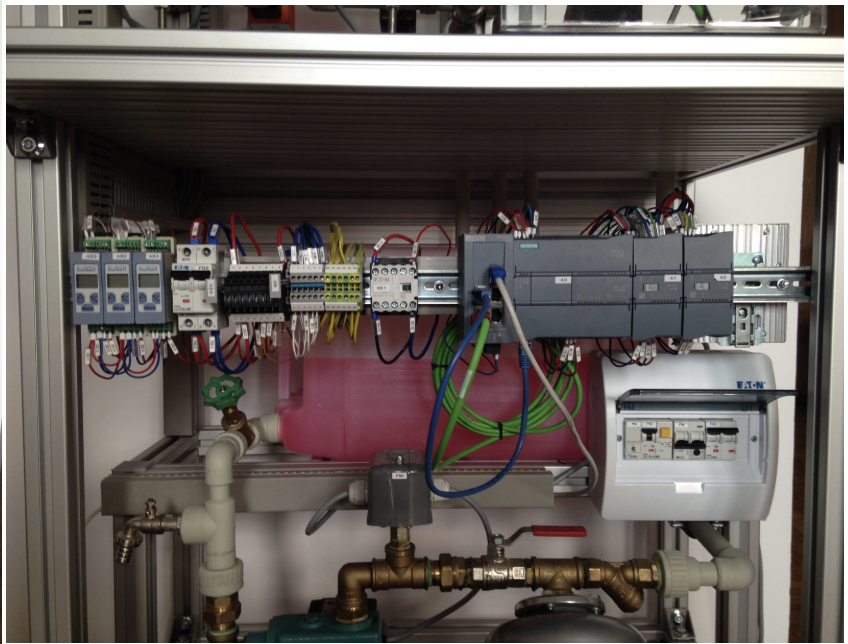
\includegraphics[width=0.5\textwidth]{media/0_2_PLC.png}
            \label{fig:zdj21}}
        % Pod figura 1
        \subfloat[Całe stanowisko (zdjęcie z konspektu)]{
            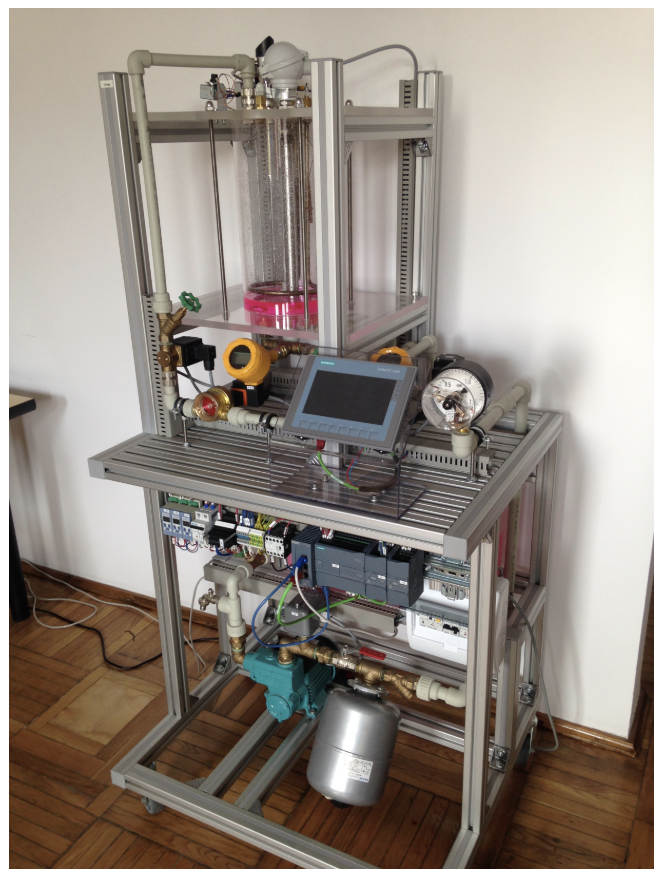
\includegraphics[width=0.5\textwidth]{media/0_1_Całe_stanowisko.png}
            \label{fig:zdj37}}
    \caption{Konfiguracja kanałów modułu}
    \label{fig:main0}
\end{figure}


\section{Konfiguracja sterownika}
Na początku ćwiczenia należało skonfigurować sterownik PLC w aplikacji \textit{TIA Portal V19} aby można było odczytać wejścia analogowe oraz zapisać wyjścia analogowe. W tym celu należało na początku należało dodać jednostkę centralną, a następnie dodać dwa moduły wejść/wyjść analogowych, które w kolejnych krokach pozwolą nam na obsługę elektrozaworów.

Po poprawnej konfiguracji wirtualny schemat układu z PLC wyglądał tak jak na zdjęciu \ref{fig:zdj1}.
\begin{figure}[H]
    \centering
    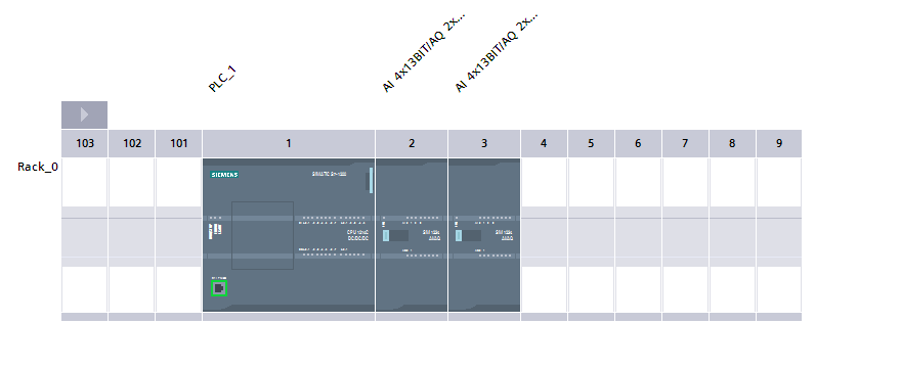
\includegraphics[width=0.5\textwidth]{media/1_1_Dodanie_modułu.png}
    \caption{Wirtualny układ z PLC}
    \label{fig:zdj1}
\end{figure}

Następnie należało ustawić poprawny adres IP, aby można było połączyć się z PLC. W tym celu należało kliknąć prawym przyciskiem myszy na jednostkę centralną i wybrać opcję \textit{Properties}, a następnie w zakładce \textit{PROFINET Interface} ustawić poprawny adres IP. Na zdjęciu \ref{fig:zdj2} przedstawione są ustawienia sieciowe PLC.
\begin{figure}[H]
    \centering
    
\includegraphics[width=0.5\textwidth]{media/1_2_Ustawienia_sieciowe_PLC.png}
    \caption{Ustawienia sieciowe PLC}
    \label{fig:zdj2}
\end{figure}

Po poprawnym wykonaniu można było połączyć się z PLC. Poprawne skonfigurowanie i wejście w tryb Online skutkowało, że Interface w aplikacji wyglądał tak jak na zdjęciu \ref{fig:zdj3}. Dzięki temu można było przejść do kolejnych kroków ćwiczenia.
\begin{figure}[H]
    \centering
    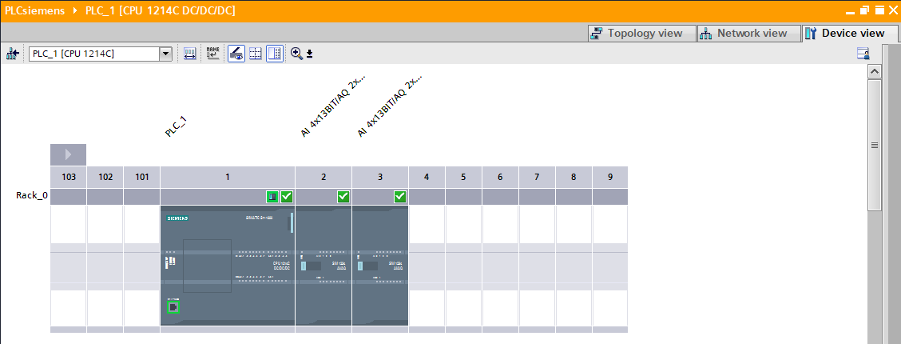
\includegraphics[width=0.5\textwidth]{media/1_3_PLC_Online.png}
    \caption{Poprawne połączenie z PLC}
    \label{fig:zdj3}
\end{figure}


\newpage
\section{Odczyt i zapis zmiennych procesowych}

\begin{figure}[H]
    \centering
    \includegraphics[width=0.5\textwidth]{media/2_1_Ustawienia_wejść_IO.png}
    \caption{DO UZUPEŁNIENIA}
    \label{fig:zdj4}
\end{figure}

\begin{figure}[H]
    \centering
    \includegraphics[width=0.5\textwidth]{media/2_2_Ustawienia_wejść_IO_OFF.png}
    \caption{DO UZUPEŁNIENIA}
    \label{fig:zdj5}
\end{figure}

\begin{figure}[H]
    \centering
    \includegraphics[width=0.5\textwidth]{media/2_3_Ustawienia_wyjść.png}
    \caption{DO UZUPEŁNIENIA}
    \label{fig:zdj6}
\end{figure}

\begin{figure}[H]
    \centering
    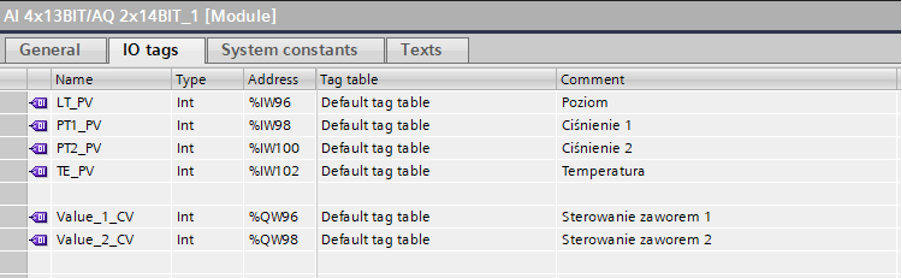
\includegraphics[width=0.5\textwidth]{media/2_4_Tagi_moduł_1.png}
    \caption{DO UZUPEŁNIENIA}
    \label{fig:zdj7}
\end{figure}

\begin{figure}[H]
    \centering
    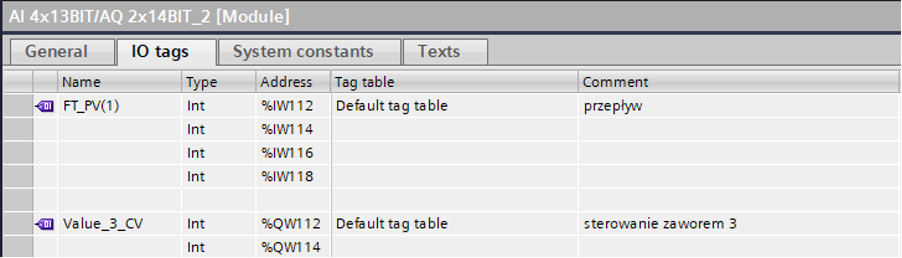
\includegraphics[width=0.5\textwidth]{media/2_5_Tagi_moduł_2.png}
    \caption{DO UZUPEŁNIENIA}
    \label{fig:zdj8}
\end{figure}

\begin{figure}[H]
    \centering
    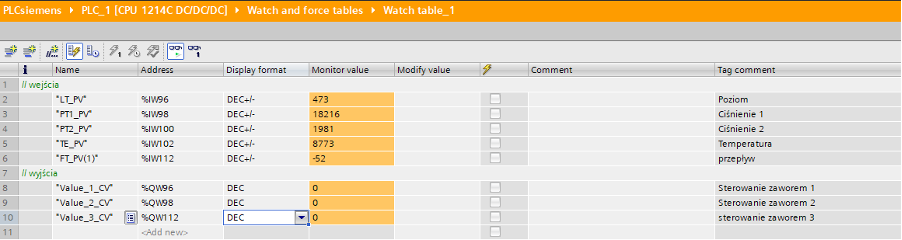
\includegraphics[width=0.5\textwidth]{media/2_6_Watch_tab_Online.png}
    \caption{DO UZUPEŁNIENIA}
    \label{fig:zdj9}
\end{figure}

\newpage
\section{Skalowanie zmiennych procesowych}
\begin{figure}[H]
    \centering
    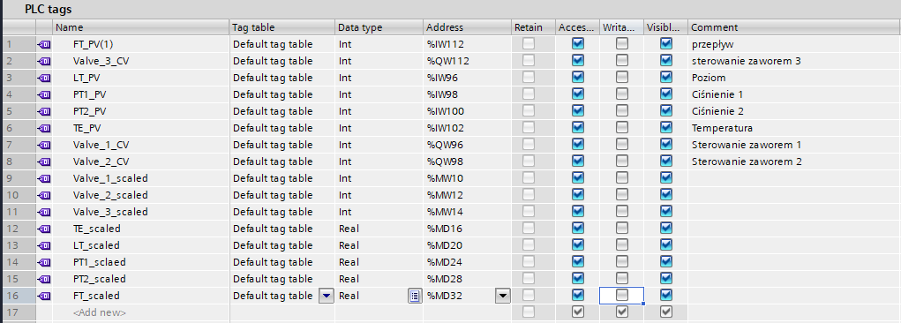
\includegraphics[width=0.5\textwidth]{media/3_1_PLC_tags_scaled.png}
    \caption{DO UZUPEŁNIENIA}
    \label{fig:zdj10}
\end{figure}

\begin{figure}[!ht]
    \centering
        % Pod figura 1
        \subfloat[DO UZUPEŁNIENIA]{    
            \centering
            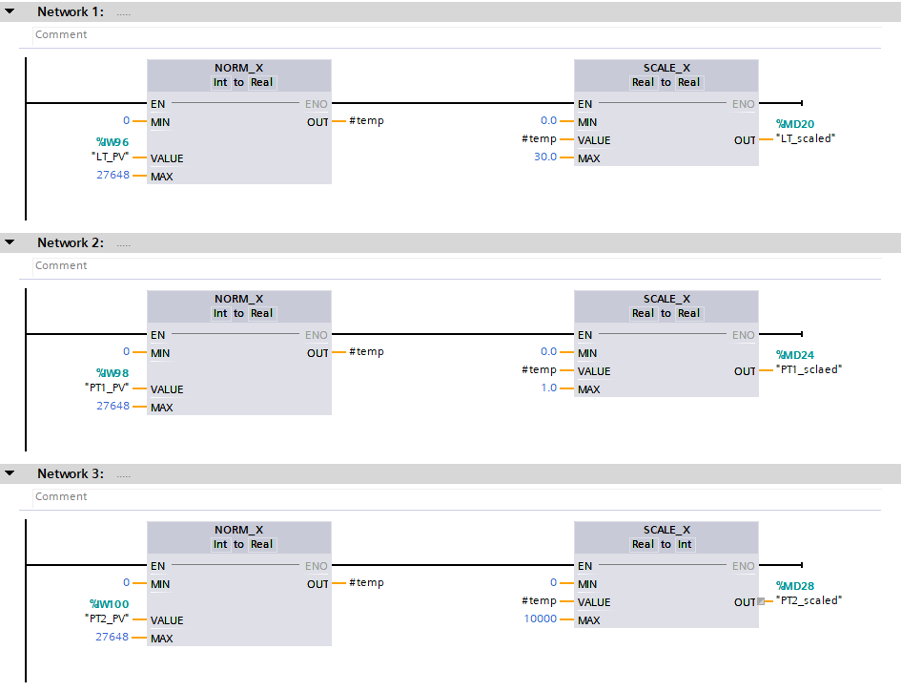
\includegraphics[width=0.5\textwidth]{media/3_2_1_PLC_logika_hej.png}
            \label{fig:zdj11}}
        % Pod figura 1
        \subfloat[DO UZUPEŁNIENIA]{
            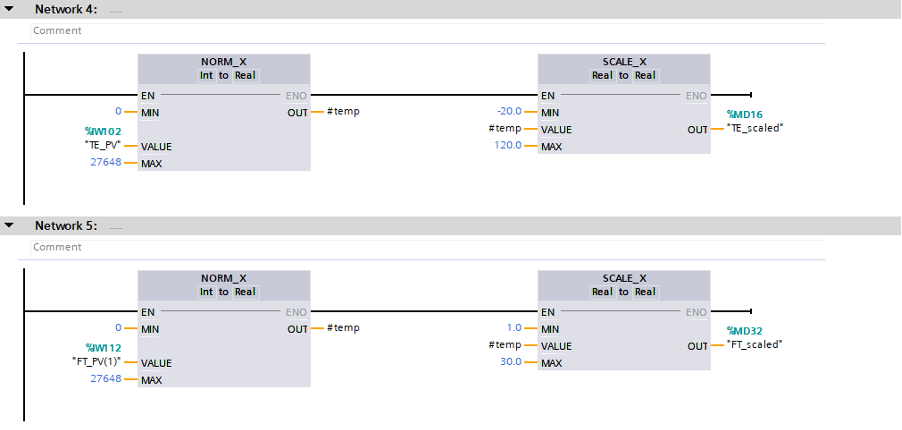
\includegraphics[width=0.5\textwidth]{media/3_2_2_PLC_logika_hej.png}
            \label{fig:zdj12}}
            \hfill
        % Pod figura 2
        \subfloat[DO UZUPEŁNIENIA]{
            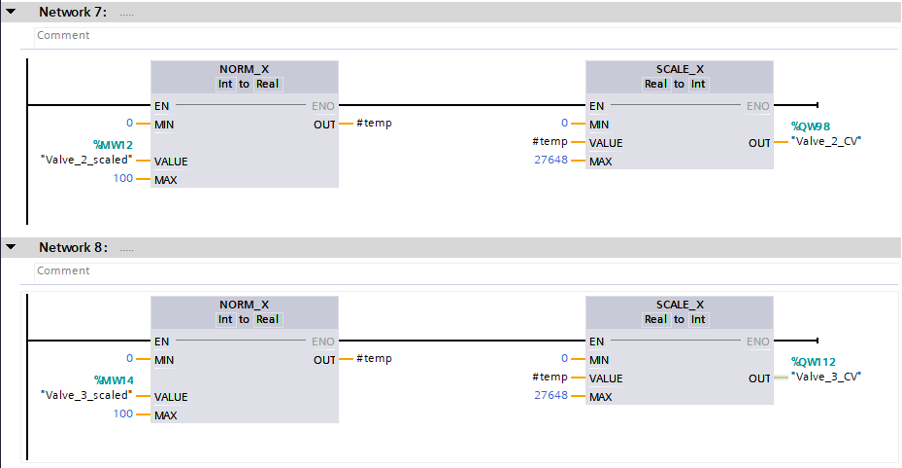
\includegraphics[width=0.5\textwidth]{media/3_2_3_PLC_logika_hej.png}
            \label{fig:zdj13}
        }
    \caption{Konfiguracja kanałów modułu}
    \label{fig:main1}
\end{figure}


\begin{figure}[H]
    \centering
    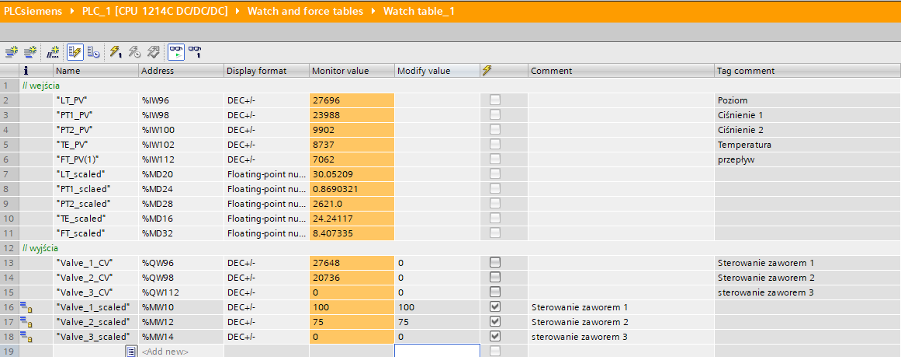
\includegraphics[width=0.5\textwidth]{media/3_3_Watch_table_online.png}
    \caption{DO UZUPEŁNIENIA}
    \label{fig:zdj14}
\end{figure}

\newpage
\section{Podsumowanie}
\end{document}
